\chapter{Chapter 1 - Theory}

In this chapter we will discuss the general model used to predict binding and cleavage. This entire work is theoretical so this chapter could be very long. Instead this chapter will contain the very fundamentals of the model, some important insights and some expressions and formulas that will be used throughout this thesis. This necessarily means more theory, insights and slight changes to the model will follow in sections outside of this one, but the fundamentals of the model will be laid out here.

%TODO Picture with definitions of certain elements. - Better and shorter than words.

\section{Definitions}
Since the model is build on the physics underlying the binding and cleaving by Cas9 it is useful to first get a simplistic understanding of what the enzyme exactly is and how it works. In figure \ref{fig:Cas9schematic} a schematic of (d)Cas9 is depicted. It shows the general shape of the enzyme and some important components.


\begin{figure}[H]
\begin{center}
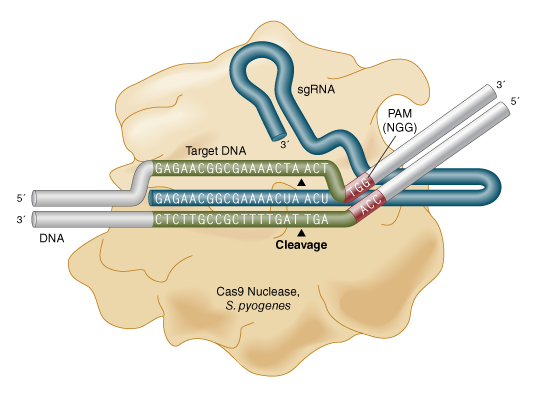
\includegraphics[width=\textwidth]{images/Cas9schematic}
\caption{Schematic of (d)Cas9}
\label{fig:Cas9schematic}
\end{center}
\end{figure}

In figure \ref{fig:Cas9schematic} several components of Cas9 are defined, we will take a closer look at what each of these is. In the schematic there are two strands of DNA (white/beige) and one strand of RNA (blue). The RNA is called sgRNA or gRNA, short for (single stranded) guide RNA. The gRNA is connected to the enzyme but it is fabricated separately and is attached later to the Cas9. Therefore the gRNA is also easily fabricated in a lab. One of the DNA strands contains the target sequence (and naturally the other contains the complement to the target sequence). Finally the DNA contains the PAM (protospacer adjacent motif) sequence. This is a sequence (NGG) just before the target sequence (sometimes called protospacer) that does not match to the gRNA but it matches to the exact shape of the enzyme. Because this sequence depends on enzymatic interactions, it is practically unchangeable.

\section{General Model}
\label{seq:generalmodel}

The model from \cite{Misha} is quite simple at its core. Cas9 binds to the DNA in essentially two ways. One section forms bonds between the target DNA and gRNA. The gRNA has a length of twenty bases. The second section forms 'bonds' between the target DNA and the protein itself, the PAM section. Once everything is bound, the PAM and all twenty bases in the gRNA, active Cas9 is able to cleave the DNA.

%\begin{figure}[H]
%\begin{center}
%\includegraphics[width=\textwidth]{images/%CRISPRCARTOON}
%\label{fig:Crispr_Cartoon}
%\caption{A simplified schematic of the various components in Cas9 while bound to the DNA.}
%\end{center}
%\end{figure}

The model used to predict binding and cleavage is analogous to a zipper. In a zipper there are separate teeth that get locked together one after another when the zipper is tightened. In a similar way the teeth let loose one set after another when the zipper is loosened. Analogous, when the DNA and Cas9 bind to each other first the PAM binds, then the first base pair of the gRNA, then the second base pair, then the third, etcetera. This continues until all twenty bases are bound to each other and only then Cas9 can cleave. Not only is the one-by-one binding of the bases similar to the one-by-one interlocking teeth of a zipper, the entire process is also reversible like a zipper. The bound bases can also one-by-one unbind from each other just like the teeth of a zipper can be separated again. The only difference here is that once the DNA is cleaved, the process can not be reversed.

\begin{figure}[H]
\begin{center}
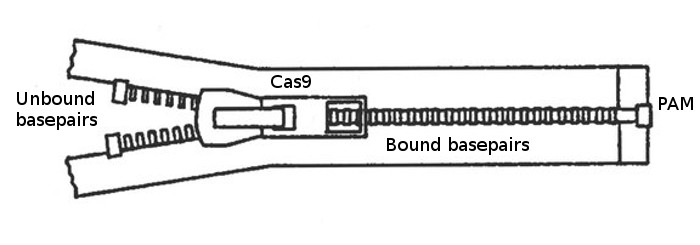
\includegraphics[width=\textwidth]{images/zipper2}
\caption{The model behaves just like a zipper.}
\label{fig:zipper}
\end{center}
\end{figure}

With this zipper model in mind we can describe the binding of Cas9 to the DNA as a number of distinct states. The first state in our model is simply unbound Cas9; the DNA and the enzyme are separate. This is similar to a zipper which is entirely separated. The second state in our model is the one where only the PAM is bound, similar to attaching the very first part of the zipper; no teeth are interlocked yet but the first connection is made and the two strands are attached to each other. %TODO Write this better
After that we have twenty states corresponding to the binding of each of the base pairs, similar to a zipper which has twenty pairs of teeth. Finally we have the very last state where the Cas9 cleaves the target DNA. This last cleaved state is special because it is irreversible. Therefore it does not have an analogous state in the zipper picture. A schematic drawing of the separate states is shown in \ref{fig:mastereqn_schematic1}.


\begin{figure}[H]
\begin{center}
\includegraphics[scale=0.35]{images/MasterEqnFlow}
\label{fig:mastereqn_schematic1}
\caption{A schematic representation of the system.}
\end{center}
\end{figure}


A well-functioning zipper is similar to the actual target of a Cas9 enzyme, called the on-target. The start of the DNA sequence of the on-target fits the PAM of Cas9 and every base on the DNA perfectly corresponds to its complement on the gRNA. An off-target however is similar to a zipper with a broken tooth somewhere along the way. Everything up to the broken tooth is similar to a well-functioning zipper but it is hard to pull the zipper over the broken tooth since the teeth will not interlock correctly. However once the zipper is pulled over the broken tooth it is again easy to tighten the rest of the zipper. This broken tooth is a mismatch on the target DNA. At first Cas9 has no way of knowing which sequences are off-targets, so it will bind to the off-target. However, somewhere along the way it will hit the mismatch. If it makes it over the mismatch it is then easy to continue further and eventually cleave the DNA, but since the mismatch is difficult to pass, the Cas9 can also simply unbind from that particular DNA sequence.

This zipper picture tells us how to think of Cas9 binding and cleavage but it does not yet allow us to predict which DNA sequences will be cleaved. To make that prediction we prescribe every state with a certain energy. We know that processes always tend to the state with the lowest possible energy. For now we will not worry about the precise values of the energies is but we can assume certain things from what we know about Cas9:

\begin{enumerate}
\item The solution state has a certain energy associated with it, but since all energy changes are relative we can set the solution energy to any value we want. Therefore only increases and decreases in energy matter.
\item A sequence with a matching PAM is more likely to cleave than a non-matching PAM. Therefore a matching PAM has a lower energy than a non-matching PAM. This is justified by the fact that we mostly measure canonical PAM sequences cleaved [SOURCE] and by the fact that Cas9 has a specific shape to recognize the canonical PAM sequence. Naturally non-canonical PAM sequences therefore have less affinity to be bound.
\item The PAM energy and therefore all subsequent energies, depend on the concentration of (d)Cas9. This is the entropic effect. Logically, if there is a surplus of Cas9 in solution, more of it will be bind to less favourable sequences.
\item Matching bases increase the likelihood of cleaving the DNA, therefore a matching base must be an energy decrease. If matching bases did not increase the chance of cleavage then almost no sequences would be cleaved in a short timeframe.
\item Non-matching bases decrease the likelihood of cleaving the DNA, therefore a mismatch must be an energy increase. This is justified because, if mismatched bases also decreased the energy then it would be favourable to cleave all sequences.
\item The process of binding one base pair involves several things. First the DNA pair must be separated, then the DNA base must turn to the RNA base and then the RNA and DNA base must bind to each other. The unbinding of the DNA base pair and the turning of the DNA base will, at first, increase the energy in the system. This is the activation energy.
\end{enumerate}

From these assumptions we can draw some general energy landscapes, as seen in figure \ref{fig:energy_landscape_cartoon}.

%TODO Maybe different figure - Move dots..
\begin{figure}[H]
\begin{center}
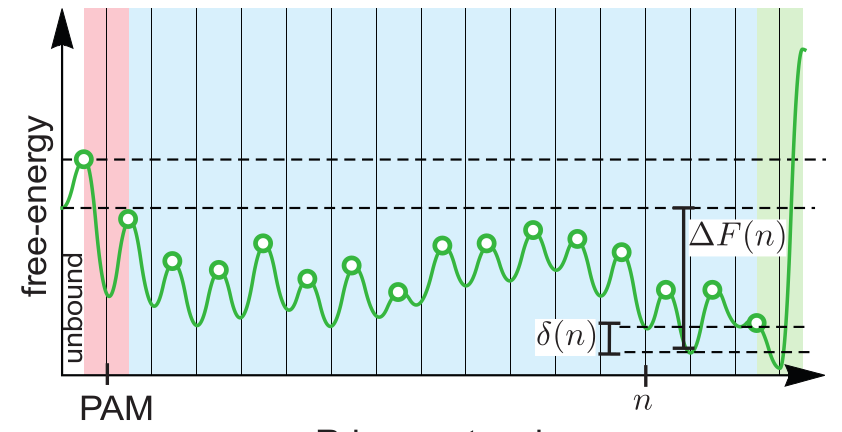
\includegraphics[width=\textwidth]{images/ENERGYLANDSCAPECARTOON}
\label{fig:energy_landscape_cartoon}
\caption{A visualization of how the energy landscape could look like.}
\end{center}
\end{figure}

At this point we know that Cas9 behaves as a sort of zipper and each state has an associated energy. It is also known that nature tends towards the lowest energy state. From this it is clear that some sequences will be cleaved; the ones with a low final energy, and some will not be cleaved; the ones with a high final energy. Similar conclusions can be drawn for binding instead of cleaving, but they are not as straightforward. For binding it is possible to have metastable states that allow stable binding, even on sequences that will never be cleaved. This is because, for cleavage the only important question is if Cas9 is able to reach the final state. For binding the question is if there are any stable states (lower energy than solution).

With this rudimentary pictuer of the zipper in mind we can create countless different models. The only thing we need to know are the energy values of each state and the rate at which dCas9 transitions between states. These energies and rates together fully describe the system, both in equilibrium and out of equilibrium.

\subsection{Equilibrium}
\label{seq:EquilTheory}

The simplest way to calculate the fraction of bound Cas9 is to assume that the entire system is in equilibrium. In equilibrium there is no evolution over time and therefore the transition rates which determine how the system evolves over time drop out of the model. If the system is in equilibrium and there are no exclusion effects then we can use Boltzmann statistics to determine the fraction of Cas9 in each available state by only knowing the energy of each state. The probability to be in a single state is as follows:

\begin{equation}
P_i = \frac{\exp{(-E_i)}}{\sum_{i=-1}^{N}\exp{(-E_i)}},
\end{equation}

where N is the total number of states available and $E_i$ is the energy of state $i$. If we consider only the solution state as unbound, then the probability of being bound ($P_b$) in equilibrium is:

\begin{equation}
P_b = \frac{\sum_{i=0}^{N}\exp{(-E_i)}}{\sum_{i=-1}^{N}\exp{(-E_i)}},
\end{equation}

where we have set 'state -1' to be the solution state. This calculation is simple and can easily be done by hand, but that is not the case if the system is out of equilibrium.

\subsection{Time dependent}
\label{sec:TimeDepTheory}

When the system is not in equilibrium a time dependency is introduced which makes the problem significantly more difficult. Not only the calculations will be harder to do but since the system evolves over time the transition rates do not drop out. As far as we know there is no exact solution to the problem when it is not in equilibrium, however we can calculate the solution numerically. To do this we solve the master equation numerically. We assume that the entire system has $N$ different states: the unbound state, the PAM bound state and one state for each subsequent base pair. Each state is able transition to the next or previous state only with a certain rate for each transition. Schematically this can be represented as in figure \ref{fig:mastereqn_schematic}. Each circle in this diagram represents a state of the system and each arrow represents a forward or a backward rate to go from a state to another.

\begin{figure}[H]
\begin{center}
\includegraphics[scale=0.35]{images/MasterEqnFlow}
\label{fig:mastereqn_schematic}
\caption{A schematic representation of the system.}
\end{center}
\end{figure}

Any particular dCas9 enzyme has a probability $P_i(t)$ to be in a specific state $i$ at a specific time  $t$. If we look at the probability $P_i(t+dt)$ to be in the state $i$ at a slightly later time $t+dt$ then the probability has changed to

\begin{equation}
P_i(t+dt) = P_i(t) - P_i(t)\cdot (\lambda_i + \mu_i)\cdot dt + \lambda_{i-1}P_{i-1}(t)\cdot dt + \mu_{i+1}P_{i+1}(t)\cdot dt,
\end{equation}

which holds as long as $dt$ is small enough to only allow a single transition. Here $\lambda_i$ is the forward rate from state $i$ to state $i+1$ and $\mu_i$ is the backward rate from state $i$ to state $i-1$. Rewriting this equation and letting $dt \rightarrow 0$ we get

\begin{equation}
\label{eq:dpdtmasteri}
\frac{\partial P_i(t)}{\partial t} = (-\lambda_i - \mu_i)P_i(t) + \lambda_{i-1}P_{i-1}(t) + \mu_{i+1}P_{i+1}(t),
\end{equation}

for $i \in [-1,N]$. Where we call state $-1$ the free state, state $0$ the state with only the PAM bound and states $1..N$ the states with bases $1..N$ bound. We can write equation \ref{eq:dpdtmasteri} in matrix form

\begin{equation}
\label{eq:mastermatrix}
\frac{\partial \vec{P}(t)}{\partial t} = M\cdot \vec{P}(t),
\end{equation}

where $M$ is the transition matrix containing the forward and backward rates. Note that we have basically rewritten the master equation in matrix form. One can easily solve this equation:

\begin{equation}
\label{eq:MasterEquationSolution}
\vec{P(t)} = exp(M\cdot t) \cdot \vec{P}(0).
\end{equation}

This gives the probability of a specific molecule to be in each state at a time $t$. In other words, this is the fraction of molecules in each state at a time $t$. Following Kramers rate theory [SOURCE] the forward and backward rates contained within the matrix $M$ are given by:

\begin{align}
\label{eq:Kramer}
k_f(i) &= k_0 \cdot exp(F_i - T_i) \\
k_b(i) &= k_0 \cdot exp(F_i - T_{i-1}),
\end{align}

with $F_i$ the free energy of state $i$ and $T_i$ the transition energy from state $i$ to state $i+1$. Therefore

\begin{equation}
k_b(i) = k_f(i-1) \cdot exp(F_{i}-F_{i-1}).
\end{equation}

The energy landscape therefore also contains information about the rates. In fact, if the energy landscape is known it is possible to calculate all forward or backward rates if all backward or forward rates are known respectively. To eliminate a lot of potential parameters we will assume for most models that the forward rates are all equal. This is a reasonable assumption since physically the molecules only feels the interaction of the forward barrier for its forward rate. This energy barrier is determined by the energy it takes to break up the DNA-DNA bond and, approximating all DNA bonds as equal, this is always the same. The only forward rate we have not assumed the same is that from solution to the first (PAM) bound state, since this can vary with concentration of dCas9 and the interaction between the PAM sequence and the protein is fundamentally different from all other bonds that are formed. Thus, if all forward rates are assumed to be constant and the same: $k_f(i) = k_f(i+1)$ for all $i \neq -1$, we can completely determine the transition matrix in equation \ref{eq:MasterEquationSolution} given two rates: the rate from solution to PAM (the on-rate) and a rate from any bound state to any other state (the attempt rate). The attempt rate is the $k_0$ factor that is shown in equations \ref{eq:Kramer}.



\section{Minimal model}
The simpelest model of all is what will be called 'the minimal model'. This model is the one which captures all our assumptions in the least amount of parameters possible. In fact it only requires three parameters: the energy gain from a match ($\epsilon C$) the energy penalty of a mismatch ($\epsilon I$) and the energy gain or penalty of the PAM ($\epsilon PAM$) to fix the energy landscape. It also contains two parameters to describe the time evolution of the system: the on-rate ($k_{on}$) and the attempt rate ($k_0$). The minimal model will build the foundation for this entire report.

The minimal model encompasses everything described in section \ref{seq:generalmodel}. To predict the binding probability of any sequence we only have one question left to answer: 'When is a Cas9 enzyme bound?' This may seem like a silly question but it is important to agree on what constitutes binding. One option is to only mark Cas9 as bound when it reached the final state in the system, meaning a fully formed R-loop. Another option is to mark Cas9 bound when the entire seed-region is bound. A third proposition could be to mark Cas9 as bound when it is simply not unbound, so every state except solution would be a 'bound state'. None of these definitions is necessarily better than any other but it is important to be consistent, even more so between theory and experiment. Therefore we will consider all states bound except the solution state. Not only does this make intuitive sense, it is also the same quantity that is measured in several experiments like \citep{PNAS} and [SOURCE]. By defining binding like this the minimal model has several features that depend mostly on the energy landscape, which is determined by the free energy parameters.

\subsection{Energy landscape}
The energy landscape of the R-loop determines the fraction of the dCas9 that will be bound in equilibrium and also determines, to an extent, how fast binding happens. As discussed before, the minimal model has three free energy parameters: one for a matching PAM, one for a matching base pair and one for a mismatching base pair. When we refer to an energy landscape we refer to the entire landscape, so for all possible states, that is predicted by these three parameters. An example landscape is shown in figure \ref{fig:examplelandscapeminmodel}.


\begin{figure}[H]
\begin{center}
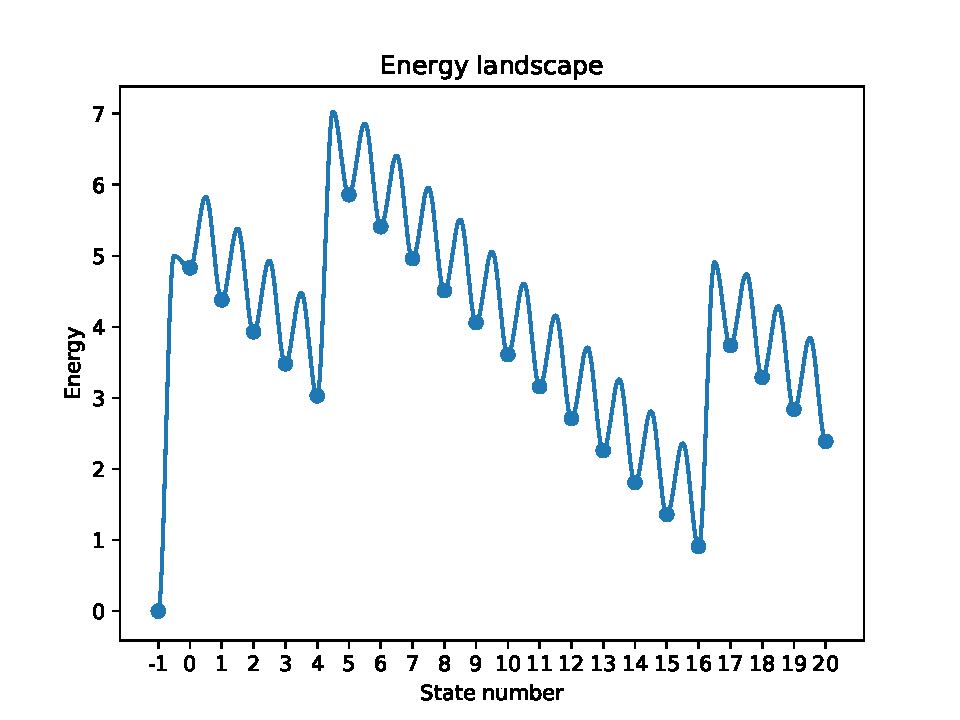
\includegraphics[width=\textwidth]{images/examplelandscapeminmodel}
\label{fig:examplelandscapeminmodel}
\caption{An example of a possible energy landscape in the minimal model. In this landscape two mismatches occur at positions five and seventeen.}
\end{center}
\end{figure}

By looking at the energy landscape it is possible to predict quite a lot about the behavior of the system. We will note several of these features and describe them by referring to several energy landscapes. These explanations will focus on building an understanding about the system as described by the minimal model, therefore they will not contain much mathematics but refer to several drawn energy landscapes instead.

\subsection{Seed region}
The first feature that is predicted by the minimal model, which is also a known feature of Cas9 is that the closer a mismatch is to the PAM, the less likely the sequence is to cleave [SOURCE]. One could assume then that the sequence is also less likely to bind than another sequence without mismatches or with mismatches far removed from the PAM. The region 'close to the PAM' is often referred to as the seed region. If there is a mismatch in this seed region binding is hard and most dCas9 will stay unbound. If instead a mismatch occurs at the end of a sequence dCas9 will readily bind to that sequence. The switch from low binding probability to high binding probability happens at the end of the seed region. This seed region can be easily identified in any energy landscape. In figure \ref{fig:seedregionexample} an energy landscape is drawn with a mismatch at position seven, while the used parameters would predict a seed region of ten base pairs.

\begin{figure}[H]
\begin{center}
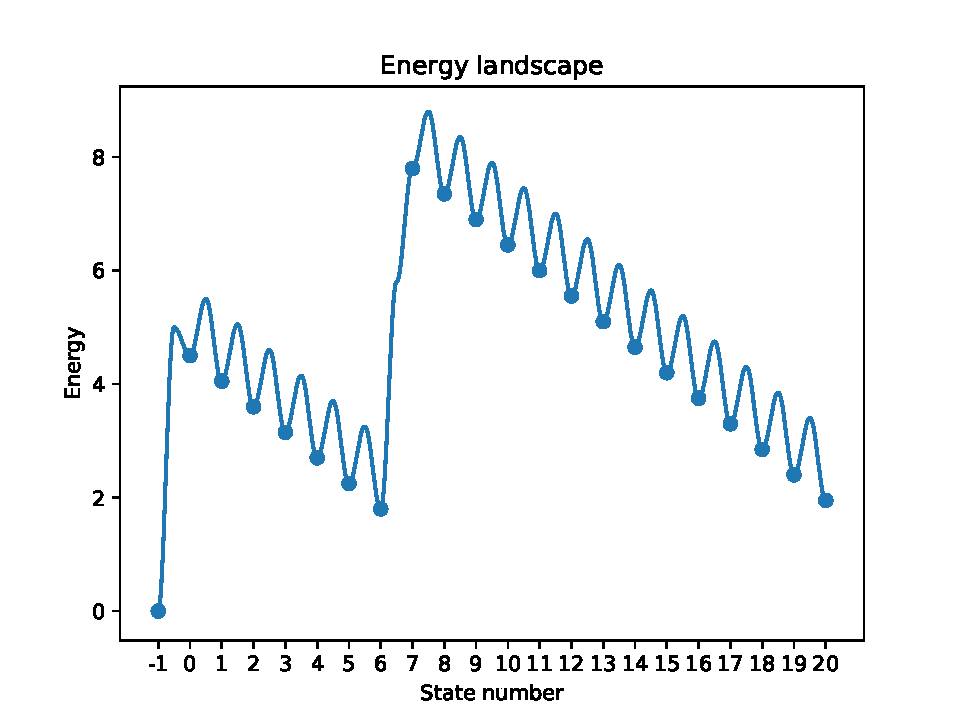
\includegraphics[width=\textwidth]{images/seedregionexample}
\label{fig:seedregionexample}
\caption{An energy landscape with a seed region of ten and a mismatch placed at position seven.}
\end{center}
\end{figure}

In figure \ref{fig:seedregionexample} the mismatch occurs within the seed region and this can easily be spotted by the fact that the mismatch occurs before any bound state becomes more favorable than the solution state. Since the solution state is still the most favorable state up to the mismatch most of the dCas9 will occupy the solution state in equilibrium. If instead the mismatch would be placed outside the seed, as in figure \ref{fig:seedregionexample2} then several bound states will have a free energy lower than the energy of the solution state. These states will be more favorable in equilibrium and therefore dCas9 will mostly occupy these states in equilibrium.

\begin{figure}[H]
\begin{center}
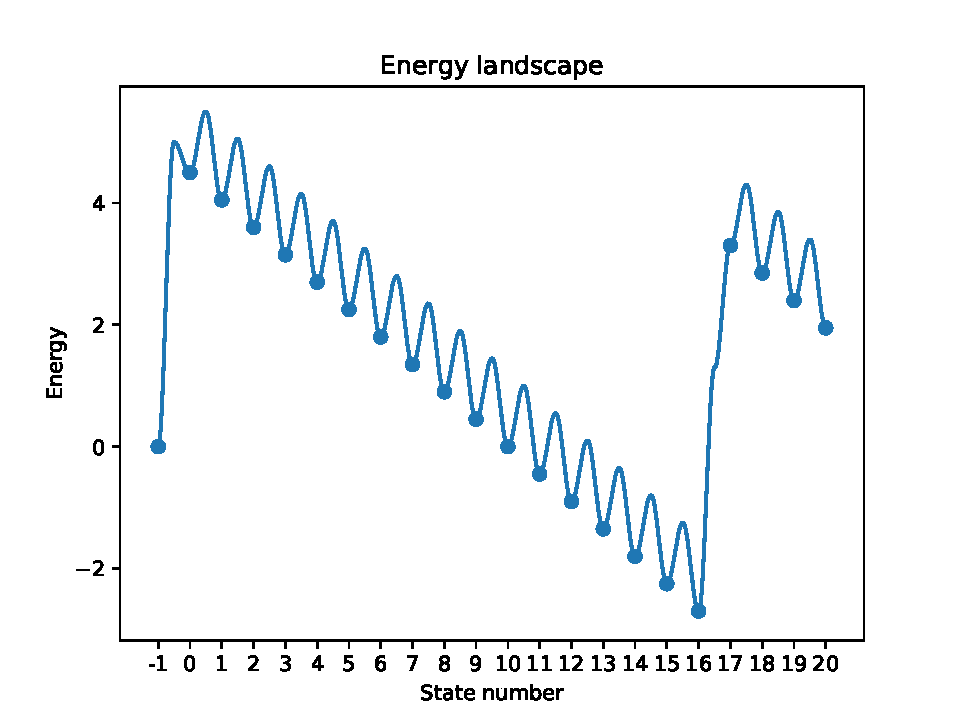
\includegraphics[width=\textwidth]{images/seedregionexample2}
\label{fig:seedregionexample2}
\caption{An energy landscape with a seed region of ten and a mismatch placed at position seventeen.}
\end{center}
\end{figure}

The length of the seed region is then determined by the values of the energy parameters $\epsilon PAM$ and $\epsilon C$. An increase in $\epsilon PAM$ lifts the energy of all states, thus making the seed region larger as it takes more matches to drop the energy below the solution energy. On the contrary a decrease in $\epsilon C$ (which is an increase in absolute value since $\epsilon C$ is negative) will make the seed region shorter, as it will take less matches to revert the energy gain from the PAM. A decrease in $\epsilon C$ has another effect on the seed region: it will make the transition from low to high binding sharper. This is because with each matching base pair the energy drops an amount $|\epsilon C$. If this is large amount then crossing the solution energy threshold can happen within a single base pair and if it is even larger then the energy of the most favorable bound state can, within one match, go from a large positive (unfavorable) energy to a large negative (favorable) energy. If there is such a sharp transition the dCas9 will go from mostly occupying the unbound state to mostly occupying the most favorable bound state if the mismatch is moved one position to the back.

Note that this definition of the seed region is fundamentally different than the definition given in \cite{Misha}, even though the same model is used. The reason for this discrepancy is that in this thesis binding instead of cleavage is considered. For cleavage the transition energies (the peaks in the energy landscape) are important while for binding the free energies (the valleys in the energy landscape) are important. For binding these free energies are important because those are the energies that the R-loops will have when they occupy those states in equilibrium. Why exactly the transition energies are important for cleavage we will leave to \citep{Misha}, for now it suffices to say that it has to do with the fact that Cas9 has to be able to make it over these energy barriers to the end of the sequence to cleave the sequence but this is not a necessity to bind the sequence.


\subsection{Minimum binding}

A second feature of the minimal model is that there will always be a minimum amount of binding for any sequence with any amount of mismatches. If we take a look at an energy landscape of a sequence containing two mismatches (shown in figure \ref{fig:minbindingexample}) it becomes clear why this is the case.

\begin{figure}[H]
\begin{center}
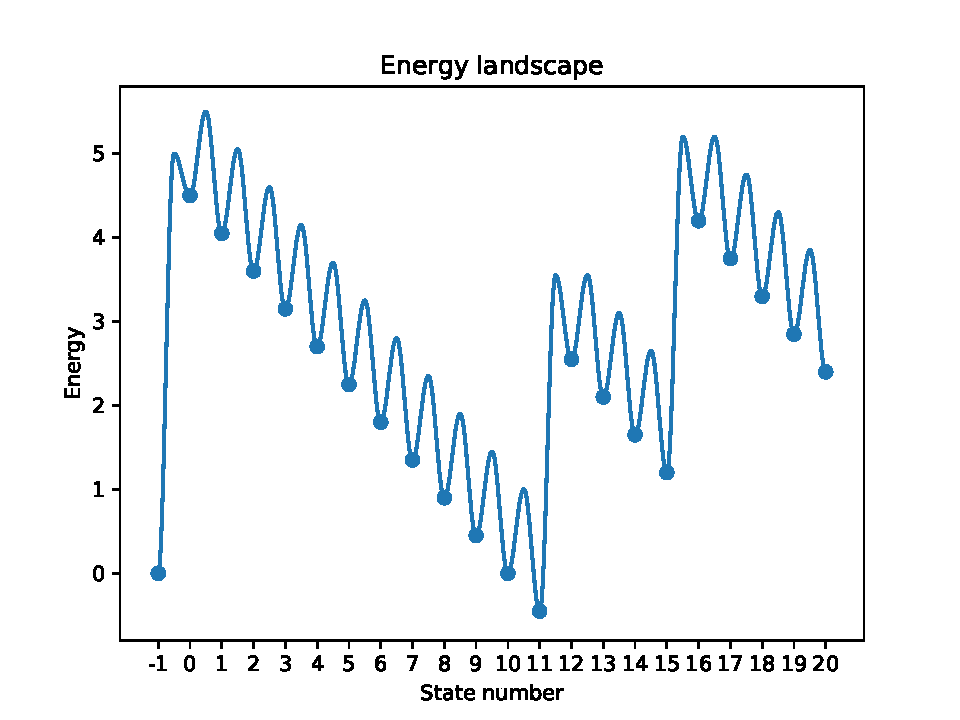
\includegraphics[width=\textwidth]{images/minbindingexample}
\label{fig:minbindingexample}
\caption{An example energy landscape containing two mismatches (positions twelve and sixteen). State eleven has lower energy than the solution state. }
\end{center}
\end{figure}

As can be seen in figure \ref{fig:minbindingexample} even though there are two mismatches some of the bound states are quite close or even below the solution energy. In equilibrium these states will have a significant amount of binding, even though the sequence contained two mismatches. There are two ways to limit this binding despite mismatched bases. The first one is quite obvious: simply add more mismatches. This will increase the energy of all subsequent states even more, therefore decreasing the amount of binding to the point where it becomes negligible. A second way is to move the mismatches closer to the PAM. Even though the total energy gained and dropped is still the same, since the parameters did not change and the amount of mismatches is constant, the fraction of bound dCas9 can still change. That the total energy gained and dropped is the same is easily proven by the fact that the final state is at the same energy, no matter where the mismatches occur. However, the states before the mismatches are not all at the same energy. Sequences that have mismatches occur nearer to the PAM contain more states where the energy increase from the mismatch has an influence. This is due to the nature of the model; where the energy of each state is the sum over the energies of all previous states plus the energy gain or penalty of the state itself. This is very easy to see if two energy landscapes with the same amount of mismatches are overlapped as in figure \ref{fig:minbindingexample2}. The sequence with mismatches more to the end clearly has more states with a lower energy, even though the final energy is the same.

\begin{figure}[H]
\begin{center}
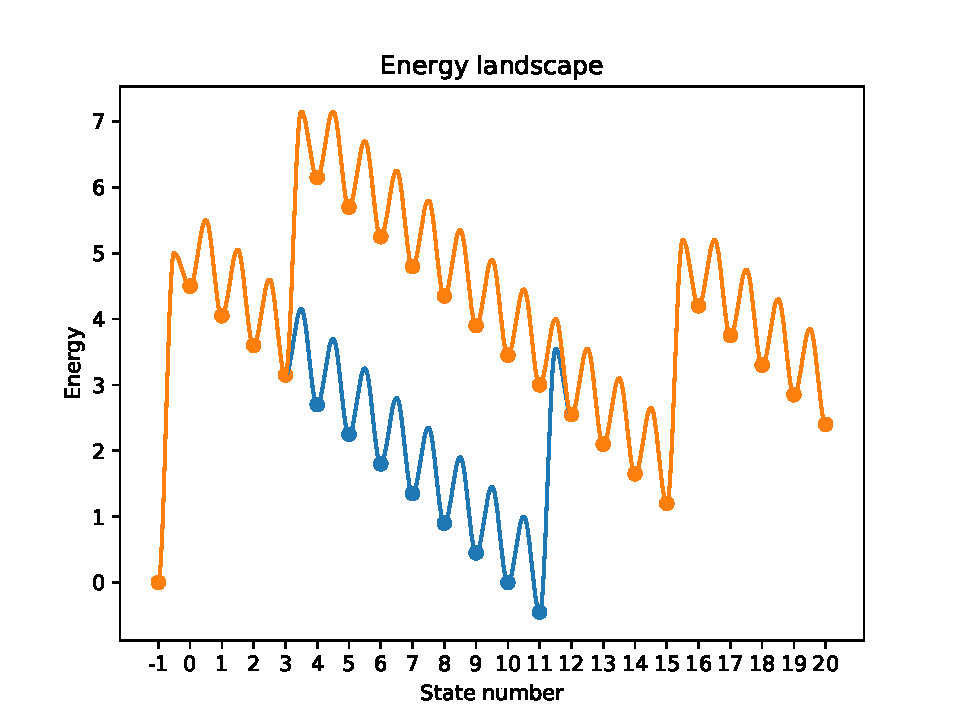
\includegraphics[width=\textwidth]{images/minbindingexample2}
\label{fig:minbindingexample2}
\caption{Two possible energy landscapes containing two mismatches each generated with the minimal model. The blue landscape is the same as in figure \ref{fig:minbindingexample}. Even though the total number of mismatches is the same, the blue energy landscape has more states with much lower energies.}
\end{center}
\end{figure}

The minimal amount of binding in equilibrium, according to the minimal model, is therefore the amount of bound dCas9 on the sequence where all mismatches occur at the very start of the R-loop. In the case of two mismatches the sequence where mismatches occur at position one and two would bind the minimum amount of dCas9 that will be bound by any sequence where in total two mismatches occur. Naturally then if the amount of mismatches increases, the minimum amount of bound dCas9 decreases.


\subsection{Maximum binding}
The minimal model not only predicts a minimum amount of bound dCas9 given a number of mismatches, it also predicts a maximum amount of bound dCas9. The reasoning is much the same as the reasoning for the minimum binding but reversed. The maximum amount of binding for a sequence with $n$ mismatches is reached when those mismatches occur in the last $n$ states. This is also very clear if we overlap two energy landscapes of two sequences with the same number of total mismatches, shown in figure \ref{fig:maxbindingexample}. The sequence which contains the later mismatches has more states with a lower energy, even though the final state again has the same energy in both cases. Since there are more states with a lower free energy, a higher fraction of dCas9 will bind to that sequence.

\begin{figure}[H]
\begin{center}
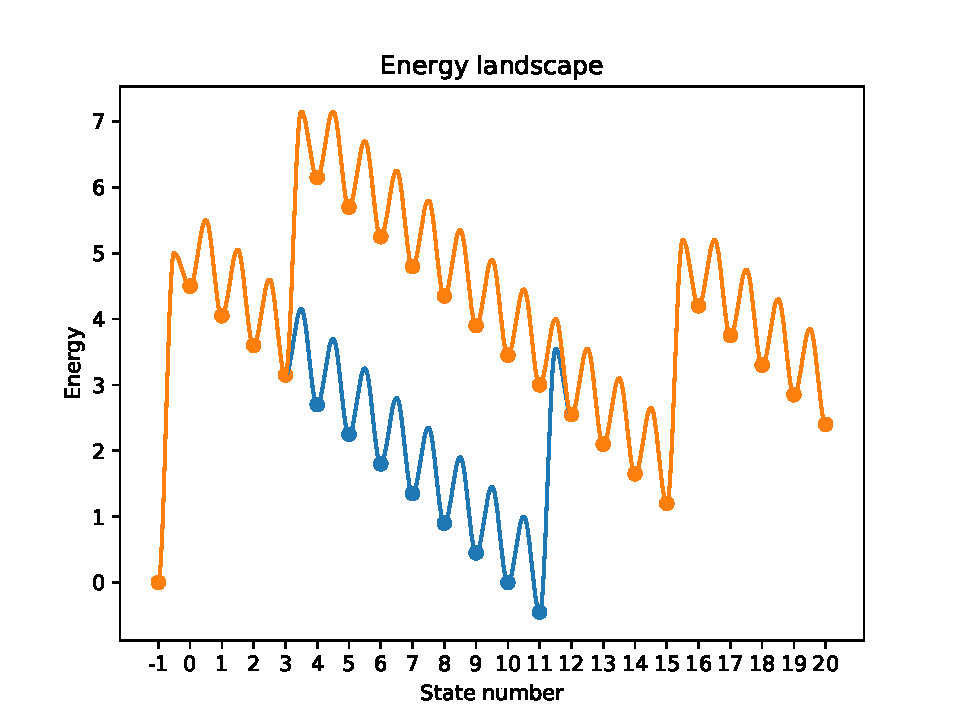
\includegraphics[width=\textwidth]{images/minbindingexample2}
\label{fig:minbindingexample}
\caption{Two possible energy landscapes containing two mismatches each generated with the minimal model. Even though the total number of mismatches is the same, the orange energy landscape has more states with much higher energies.}
\end{center}
\end{figure}

In the same way as with the minimum binding the maximum amount of binding can be decreased in two ways. Firstly it is possible to increase the number of mismatches. Secondly it is possible to move the mismatches to the end of the sequence. No sequence with $n$ mismatches can therefore bind more dCas9 than a sequence with those $n$ mismatches at the final $n$ positions.

\subsection{Pair region}
\label{sec:TheoryPair}

The previous features were all easily demonstrated by looking at the energy landscape since they all depended on single things. The last feature of the minimal model that will be discussed here is different because it depends on an interaction within the energy landscape. The pair region refers to a sort of second-seed region. The seed region discussed before is the region where a mismatch prohibits much binding of any sort and can be identified in the energy landscape as the point where the energy of the matching bases dips below the energy of the solution. Consider now that the effect of a mismatch is not as large as in figure \ref{fig:seedregionexample} but smaller as in figure \ref{fig:pairexample1}. Then the final states are still below the energy of the solution state and therefore there will still be significant binding in equilibrium, even though there is a mismatch in the seed.

\begin{figure}[H]
\begin{center}
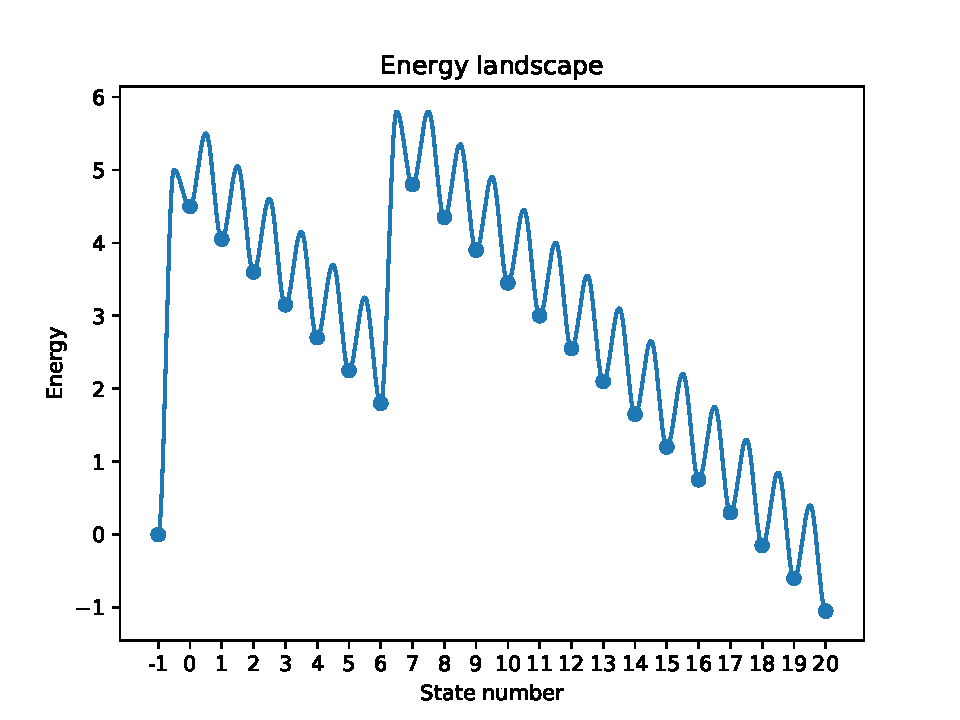
\includegraphics[width=\textwidth]{images/pairexample1}
\label{fig:pairexample1}
\caption{A possible energy landscape with a seed mismatch which still contains stable bound states.}
\end{center}
\end{figure}

This changes if a second mismatch is added. If the second mismatch is placed directly behind the first one then there may be no state below the solution state, as shown in figure \ref{fig:pairexample2}, however if the mismatches are spaced apart a similar situation as with the PAM occurs. The energy of the R-loop starts near the energy of the solution state and is increased. This increase is now due to a mismatch instead of the PAM but there is an increase nonetheless. Then there may follow a number of matching base pairs which create a second opportunity to decrease the energy below the energy of the solution. If the second mismatch is placed after this second-seed region then there will be a state or several states which are again more favorable than the solution state, therefore increasing the amount of binding significantly. This second seed region is named the pair region. An example of a sequence where the second mismatch is placed after the pair region is shown in figure \ref{fig:pairexample3}.

\begin{figure}[H]
\begin{center}
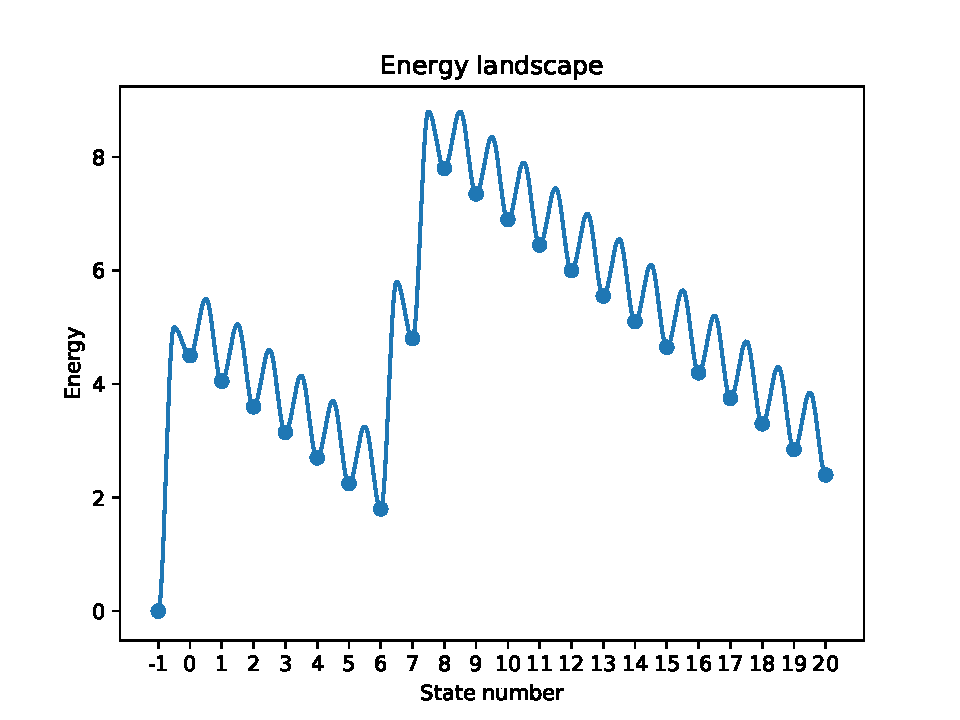
\includegraphics[width=\textwidth]{images/pairexample2}
\label{fig:pairexample2}
\caption{A possible energy landscape with a double seed mismatch so that there are no stable bound states.}
\end{center}
\end{figure}

\begin{figure}[H]
\begin{center}
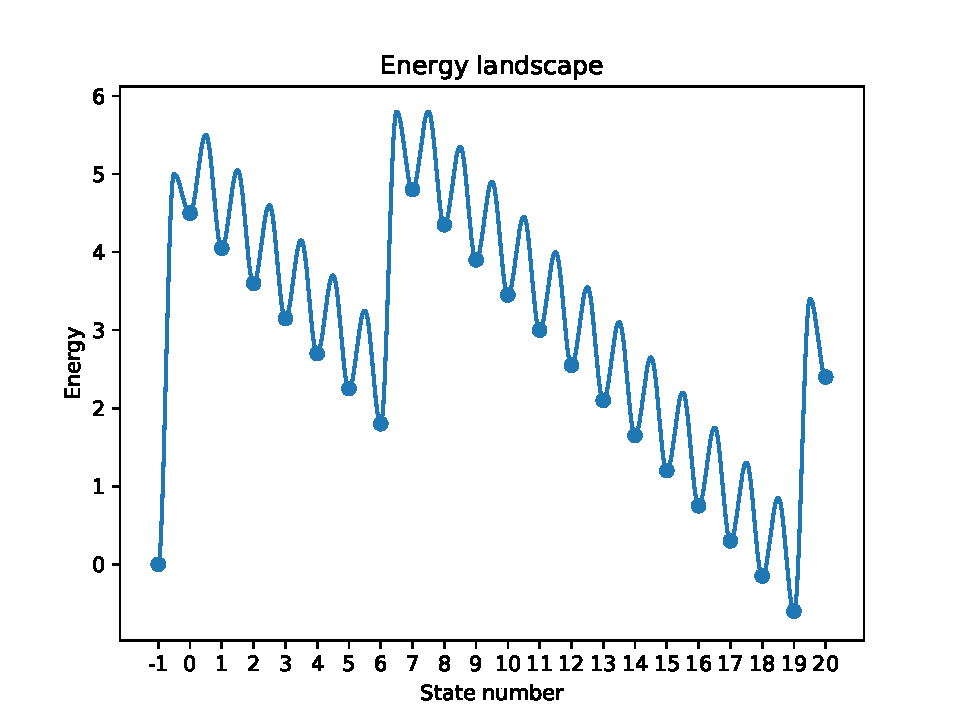
\includegraphics[width=\textwidth]{images/pairexample3}
\label{fig:pairexample3}
\caption{A possible energy landscape with a seed mismatch and a mismatch at the end so that the second mismatch does not prohibit binding even though there is a seed mismatch. The second mismatch is placed after the pair region.}
\end{center}
\end{figure}

The pair region is very similar to the seed region. It gets larger as the energy increase which causes it gets larger; the mismatch energy penalty in the case of the pair region. It gets smaller and sharper as the energy gain from a match becomes larger, all for the same reasons as for the seed region. In theory there can be multiple pair regions if there are more than two mismatches present, however the length of the gRNA is limited so there can not be arbitrarily many pair regions without extending the gRNA.























